\documentclass[12pt,a4paper]{article}

% ─── Page Layout ───────────────────────────────────────────────────────────────
\usepackage[a4paper, margin=0.8in, headheight=14pt]{geometry}

% ─── Fonts (XeLaTeX) ───────────────────────────────────────────────────────────
\usepackage{fontspec}
\usepackage{unicode-math}
\setmainfont{TeX Gyre Pagella}
\setmonofont[Scale=0.88]{TeX Gyre Cursor}
\setmathfont{Latin Modern Math}

% ─── Packages ──────────────────────────────────────────────────────────────────
\usepackage{xcolor}
\usepackage{colortbl}
\usepackage{titlesec}
\usepackage{enumitem}
\usepackage{tabularx}
\usepackage{booktabs}
\usepackage{array}
\usepackage{amsmath}
\usepackage{tikz}
\usetikzlibrary{shapes.geometric, arrows.meta, positioning, calc, fit, decorations.pathreplacing}
\usepackage{tcolorbox}
\tcbuselibrary{skins, breakable}
\usepackage{hyperref}
\usepackage{fancyhdr}
\usepackage{graphicx}
\usepackage{microtype}
\hyphenpenalty=10000
\exhyphenpenalty=10000
\sloppy
\usepackage{caption}
\usepackage{setspace}
\usepackage{multirow}
\usepackage{tocloft}

% ─── Q&A helper ────────────────────────────────────────────────────────────────
\newcommand{\Q}[1]{\textbf{#1}\par\noindent\ignorespaces}

% ─── Colour Palette ────────────────────────────────────────────────────────────
\definecolor{myred}{RGB}{196,30,58}
\definecolor{mydark}{RGB}{30,30,50}
\definecolor{mygreen}{RGB}{14,120,80}
\definecolor{myteal}{RGB}{0,130,140}
\definecolor{myamber}{RGB}{180,100,0}
\definecolor{mypurple}{RGB}{100,30,160}
\definecolor{mygray}{RGB}{246,247,249}
\definecolor{mgframe}{RGB}{180,185,200}
\definecolor{watermark}{RGB}{145,150,170}
\definecolor{hdrred}{RGB}{250,232,235}
\definecolor{hdrgreen}{RGB}{220,244,233}
\definecolor{hdrteal}{RGB}{220,242,244}
\definecolor{hdramber}{RGB}{253,242,215}
\definecolor{hdrpurple}{RGB}{238,228,255}
\definecolor{hdrgray}{RGB}{238,240,245}
\definecolor{rowalt}{RGB}{250,251,253}

% ─── Section Formatting ────────────────────────────────────────────────────────
\titleformat{\section}
  {\large\bfseries\color{myred}}{\thesection.}{0.5em}{}
  [\vspace{1pt}{\color{myred}\rule{\linewidth}{0.8pt}}]
\titleformat{\subsection}
  {\normalsize\bfseries\color{myteal}}{\thesubsection}{0.5em}{}
\titlespacing*{\section}{0pt}{18pt}{7pt}
\titlespacing*{\subsection}{0pt}{11pt}{4pt}

% ─── Paragraph ─────────────────────────────────────────────────────────────────
\setlength{\parindent}{0pt}
\setlength{\parskip}{4pt}

% ─── TOC Styling ───────────────────────────────────────────────────────────────
\renewcommand{\cfttoctitlefont}{\large\bfseries\color{myred}}
\renewcommand{\cftaftertoctitle}{\par\noindent{\color{myred}\rule{\linewidth}{0.8pt}}}
\setlength{\cftbeforetoctitleskip}{0pt}
\setlength{\cftaftertoctitleskip}{6pt}
\renewcommand{\cftsecfont}{\normalsize\bfseries\color{mydark}}
\renewcommand{\cftsecpagefont}{\normalsize\bfseries\color{mydark}}
\renewcommand{\cftsecleader}{\cftdotfill{\cftdotsep}}
\setlength{\cftbeforesecskip}{7pt}
\renewcommand{\cftsubsecfont}{\small\color{mydark}}
\renewcommand{\cftsubsecpagefont}{\small\color{mydark}}
\setlength{\cftbeforesubsecskip}{3pt}
\setlength{\cftsubsecindent}{1.4em}

% ─── Table helpers ─────────────────────────────────────────────────────────────
\renewcommand{\arraystretch}{1.45}
\setlength{\tabcolsep}{6pt}
\arrayrulecolor{mydark}
\newcolumntype{B}[1]{>{\small\bfseries\raggedright\arraybackslash}m{#1}}
\newcolumntype{Y}{>{\small\raggedright\arraybackslash}X}
\renewcommand{\tabularxcolumn}[1]{m{#1}}

% ─── Header / Footer ───────────────────────────────────────────────────────────
\pagestyle{fancy}
\fancyhf{}
\fancyhead[L]{\small\color{myred}\textbf{OE-EC604B}\;\color{mydark}--- Operating System}
\fancyhead[R]{\small\color{myteal}\textbf{Module 3 Notes}}
\fancyfoot[C]{\small\color{mydark}\thepage}
\fancyfoot[R]{\small\color{watermark}\textit{\copyright\ Biraj}}
\renewcommand{\headrulewidth}{0.5pt}
\renewcommand{\footrulewidth}{0.3pt}

% ─── Hyperref ──────────────────────────────────────────────────────────────────
\hypersetup{
  colorlinks=true, linkcolor=myteal, urlcolor=myteal,
  pdfauthor={Biraj Sarkar},
  pdftitle={OE-EC604B --- Module 3 Notes}
}

% ─── tcolorbox styles ──────────────────────────────────────────────────────────
\tcbset{
  tikzbox/.style={
    colback=mygray, colframe=mgframe, boxrule=0.6pt, arc=4pt,
    left=8pt, right=8pt, top=6pt, bottom=6pt,
    colbacktitle=mgframe, coltitle=mydark,
    fonttitle=\small\bfseries
  },
  defbox/.style={
    colback=hdrgreen, colframe=mygreen, boxrule=0.8pt, arc=4pt,
    left=9pt, right=9pt, top=6pt, bottom=6pt,
    colbacktitle=mygreen, coltitle=white,
    fonttitle=\small\bfseries
  },
  formulabox/.style={
    colback=hdrteal, colframe=myteal, boxrule=0.8pt, arc=4pt,
    left=9pt, right=9pt, top=7pt, bottom=7pt,
    colbacktitle=myteal, coltitle=white,
    fonttitle=\small\bfseries
  },
  examplebox/.style={
    colback=hdramber, colframe=myamber, boxrule=0.8pt, arc=4pt,
    left=9pt, right=9pt, top=6pt, bottom=6pt,
    colbacktitle=myamber, coltitle=white,
    fonttitle=\small\bfseries
  },
  masonbox/.style={
    colback=hdrpurple, colframe=mypurple, boxrule=0.8pt, arc=4pt,
    left=9pt, right=9pt, top=6pt, bottom=6pt,
    colbacktitle=mypurple, coltitle=white,
    fonttitle=\small\bfseries
  },
  exambox/.style={
    colback=hdrpurple, colframe=mypurple, boxrule=1pt, arc=5pt,
    left=10pt, right=10pt, top=8pt, bottom=8pt,
    colbacktitle=mypurple, coltitle=white,
    fonttitle=\bfseries,
    breakable, title after break={\textbf{Frequently Asked / Viva Questions (contd.)}}}
}
% Make all boxes breakable across pages
\tcbset{breakable}

% ─── TikZ styles ───────────────────────────────────────────────────────────────
\tikzset{
  block/.style={rectangle, draw=myteal, fill=hdrteal,
    text width=2.4cm, align=center, minimum height=0.95cm,
    font=\small, rounded corners=3pt, line width=0.7pt},
  redblock/.style={rectangle, draw=myred, fill=hdrred,
    text width=2.4cm, align=center, minimum height=0.95cm,
    font=\small, rounded corners=3pt, line width=0.7pt},
  greenblock/.style={rectangle, draw=mygreen, fill=hdrgreen,
    text width=2.4cm, align=center, minimum height=0.95cm,
    font=\small, rounded corners=3pt, line width=0.7pt},
  amberblock/.style={rectangle, draw=myamber, fill=hdramber,
    text width=2.4cm, align=center, minimum height=0.95cm,
    font=\small, rounded corners=3pt, line width=0.7pt},
  purpblock/.style={rectangle, draw=mypurple, fill=hdrpurple,
    text width=2.4cm, align=center, minimum height=0.95cm,
    font=\small, rounded corners=3pt, line width=0.7pt},
  sumjunc/.style={circle, draw=myamber, fill=hdramber,
    minimum size=0.62cm, font=\small, line width=0.8pt},
  arrow/.style={-Stealth, thick, color=mydark},
  redarrow/.style={-Stealth, thick, color=myred},
  line/.style={thick, color=mydark}
}

% ═══════════════════════════════════════════════════════════════════════════════
\begin{document}
% ═══════════════════════════════════════════════════════════════════════════════

\begin{center}
  {\LARGE\bfseries\color{myred} OE-EC604B --- Operating System}\\[5pt]
  {\normalsize\color{mydark} Semester VI \quad$\bullet$\quad 3L:0T:0P \quad$\bullet$\quad 3 Credits}\\[3pt]
  {\normalsize\color{myteal}\textbf{Module 3 Exam Notes: Concurrent Processes}}\\[3pt]
  {\small\color{mydark} CGEC \;$|$\; B.Tech ECE (2023--27) \;$|$\; \textit{Biraj Sarkar}}
\end{center}
\vspace{2pt}
\noindent{\color{myred}\rule{\linewidth}{1.5pt}}
\vspace{2pt}

\hypersetup{linkcolor=mydark}
\tableofcontents
\hypersetup{linkcolor=myteal}
\newpage

% ===============================================================================
\section{Process Concept and Lifecycle States}
% ===============================================================================

A \textbf{process} is a program in execution. It represents the unit of work in a modern time-sharing system.

\subsection{Process Control Block (PCB)}
Each process is represented in the operating system by a \textbf{Process Control Block (PCB)} (also called a task control block). The PCB contains:
\begin{itemize}[leftmargin=*, itemsep=3pt]
  \item \textbf{Process State:} New, ready, running, waiting, or terminated.
  \item \textbf{Program Counter (PC):} Address of the next instruction to execute.
  \item \textbf{CPU Registers:} Accumulators, index registers, stack pointers.
  \item \textbf{CPU-Scheduling Information:} Process priority, pointers to scheduling queues.
  \item \textbf{Memory-Management Information:} Page tables or segment tables.
  \item \textbf{Accounting Information:} CPU time used, time limits.
  \item \textbf{I/O Status Information:} List of open files, allocated I/O devices.
\end{itemize}

\subsection{Process States and Transitions}

\begin{tcolorbox}[tikzbox, title={Process State Transition Diagram}]
\centering
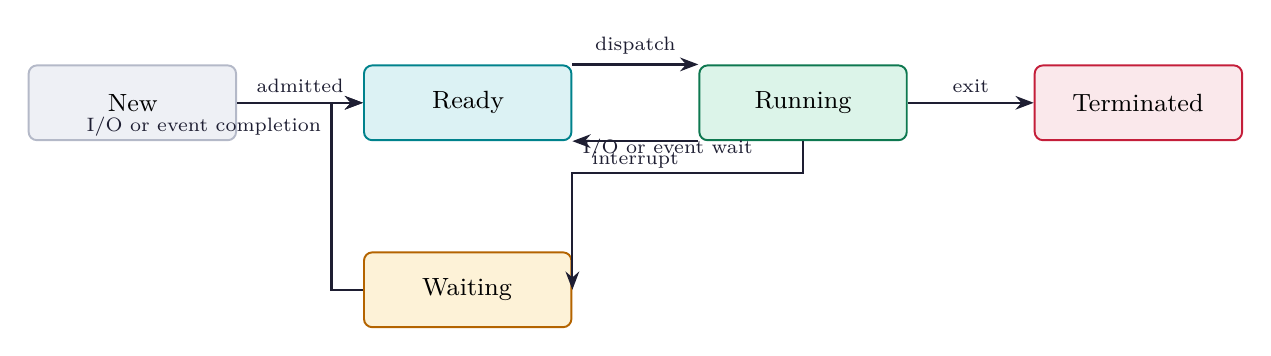
\begin{tikzpicture}[node distance=1.1cm and 1.8cm, thick, font=\small]
  \node[block, fill=hdrgray, draw=mgframe] (new) {New};
  \node[block, right=1.6cm of new, fill=hdrteal, draw=myteal] (ready) {Ready};
  \node[block, right=1.6cm of ready, fill=hdrgreen, draw=mygreen] (running) {Running};
  \node[block, below=1.4cm of ready, fill=hdramber, draw=myamber] (waiting) {Waiting};
  \node[block, right=1.6cm of running, fill=hdrred, draw=myred] (terminated) {Terminated};

  \draw[arrow] (new) -- node[above, font=\scriptsize] {admitted} (ready);
  \draw[arrow] (ready.north east) -- node[above, font=\scriptsize] {dispatch} (running.north west);
  \draw[arrow] (running.south west) -- node[below, font=\scriptsize] {interrupt} (ready.south east);
  \draw[arrow] (running) -- node[above, font=\scriptsize] {exit} (terminated);
  \draw[arrow] (running.south) -- ++(0,-0.4) -| node[right, font=\scriptsize, midway, yshift=0.3cm] {I/O or event wait} (waiting.east);
  \draw[arrow] (waiting.west) -- ++(-0.4,0) |- node[left, font=\scriptsize, midway, yshift=-0.3cm] {I/O or event completion} (ready.west);
\end{tikzpicture}
\end{tcolorbox}

% ===============================================================================
\section{Process Generation \& Scheduling Queues}
% ===============================================================================

\subsection{Process Generation (\texttt{fork()} and \texttt{exec()})}
\begin{itemize}[leftmargin=*, itemsep=3pt]
  \item \textbf{\texttt{fork()} System Call:} Creates a new, child process that is a duplicate of the parent process.
  \begin{itemize}[leftmargin=*, itemsep=2.5pt, topsep=0pt]
    \item In the parent process, \texttt{fork()} returns the PID of the child.
    \item In the child process, \texttt{fork()} returns \texttt{0}.
    \item If the call fails, it returns \texttt{-1}.
  \end{itemize}
  \item \textbf{\texttt{exec()} System Call:} Replaces the process's memory space with a new executable program, changing the active program counter.
\end{itemize}

\subsection{OS Schedulers}
\begin{itemize}[leftmargin=*, itemsep=3pt]
  \item \textbf{Long-Term Scheduler (Job Scheduler):} Selects processes from the pool (disk) and loads them into memory for execution. Controls the \textbf{degree of multiprogramming}.
  \item \textbf{Short-Term Scheduler (CPU Scheduler):} Selects from the processes in memory that are ready to execute and allocates the CPU to one of them. Executes extremely fast.
  \item \textbf{Medium-Term Scheduler:} Temporarily removes processes from memory (swapping) to reduce the degree of multiprogramming and free up RAM.
\end{itemize}

% ===============================================================================
\section{Inter-Process Communication (IPC)}
% ===============================================================================

Processes executing concurrently may be independent or cooperating. Cooperating processes require \textbf{Inter-Process Communication (IPC)}:
1. \textbf{Shared Memory:} A region of memory is established that cooperating processes can read and write to. Fast, but requires manual synchronization to prevent race conditions.
2. \textbf{Message Passing:} Processes exchange messages via the OS kernel without sharing memory space. Easier to implement but slower due to system calls.

% ===============================================================================
\section{Process Synchronization and Critical Section}
% ===============================================================================

A \textbf{race condition} occurs when multiple processes access and manipulate the same data concurrently, and the outcome of the execution depends on the particular order in which the access takes place.

\subsection{The Critical Section Problem}
The \textbf{Critical Section} is a code segment in which a process accesses shared resources.

\begin{tcolorbox}[defbox, title={\textbf{Three Requirements for a Critical Section Solution}}]
1. \textbf{Mutual Exclusion:} If process $P_i$ is executing in its critical section, no other processes can execute in their critical sections.
2. \textbf{Progress:} If no process is executing in its critical section and some processes wish to enter, only those processes not executing in their remainder sections can participate in deciding which process enters next.
3. \textbf{Bounded Waiting:} There must be a limit on the number of times other processes can enter their critical sections after a process has made a request to enter, before that request is granted.
\end{tcolorbox}

\subsection{Semaphores}
A \textbf{Semaphore} is an integer variable $S$ that, apart from initialization, is accessed only through two standard atomic operations: \texttt{wait()} (or P) and \texttt{signal()} (or V).

\begin{tcolorbox}[formulabox, title={\textbf{Semaphore Atomic Implementations}}]
\begin{verbatim}
void wait(Semaphore S) {
    while (S <= 0); // Busy wait (or block process in list)
    S--;
}

void signal(Semaphore S) {
    S++;
}
\end{verbatim}
\begin{itemize}[leftmargin=*, itemsep=3pt]
  \item \textbf{Binary Semaphore (Mutex):} Value can be either 0 or 1. Used for mutual exclusion.
  \item \textbf{Counting Semaphore:} Value ranges over an unrestricted integer domain. Used for resource allocation.
\end{itemize}
\end{tcolorbox}

\subsection{Classical Synchronization Problems}

\subsubsection{Bounded-Buffer (Producer-Consumer) Problem}
Uses semaphores to coordinate a shared buffer of size $N$:
\begin{itemize}[leftmargin=*, itemsep=3pt]
  \item \texttt{mutex} (binary, initial = 1): Protects the buffer insertion/removal.
  \item \texttt{empty} (counting, initial = $N$): Tracks empty buffer slots.
  \item \texttt{full} (counting, initial = 0): Tracks full buffer slots.
\end{itemize}

\subsubsection{Readers-Writers Problem}
Ensures multiple readers can access data concurrently, but only one writer can access it exclusively:
\begin{itemize}[leftmargin=*, itemsep=3pt]
  \item \texttt{rw\_mutex} (binary, initial = 1): Protects critical resource for writers.
  \item \texttt{mutex} (binary, initial = 1): Protects modification of \texttt{read\_count} variable.
\end{itemize}

\subsubsection{Dining Philosophers Problem}
Represents resource allocation challenges among concurrent processes. 5 philosophers sit around a table with 5 chopsticks. Each needs 2 chopsticks to eat. Prone to deadlock if everyone picks up their left chopstick simultaneously.

\subsection{Monitors}
A \textbf{Monitor} is an abstract data type that encapsulates private data and procedures, ensuring that only one process can execute inside the monitor at any given time, preventing synchronization errors automatically.

\newpage
% ===============================================================================
% MANDATORY QUICK REVISION PAGE
% ===============================================================================
\begin{center}
  {\large\bfseries\color{myred} Quick Revision --- Module 3}\\[3pt]
  {\small\color{mydark} Concurrent Processes $|$ OE-EC604B}
\end{center}
\noindent{\color{myred}\rule{\linewidth}{1.2pt}}
\vspace{4pt}

\begin{tcolorbox}[formulabox, title={\textbf{Producer-Consumer Semaphore Code}}]
\begin{tabularx}{\linewidth}{X X}
\textbf{Producer Process:} & \textbf{Consumer Process:} \\
\texttt{do \{} & \texttt{do \{} \\
\texttt{  // produce item} & \texttt{  wait(full);} \\
\texttt{  wait(empty);} & \texttt{  wait(mutex);} \\
\texttt{  wait(mutex);} & \texttt{  // remove item from buffer} \\
\texttt{  // add item to buffer} & \texttt{  signal(mutex);} \\
\texttt{  signal(mutex);} & \texttt{  signal(empty);} \\
\texttt{  signal(full);} & \texttt{  // consume item} \\
\texttt{\} while (true);} & \texttt{\} while (true);}
\end{tabularx}
\end{tcolorbox}

\begin{tcolorbox}[defbox, title={\textbf{One-Line Definitions}}]
\begin{itemize}[leftmargin=*, itemsep=2.5pt, topsep=0pt]
  \item \textbf{Process:} A program in execution containing program counter, stack, data, and registers.
  \item \textbf{PCB:} Process Control Block; kernel data structure storing all attributes of a process.
  \item \textbf{Context Switch:} Saving CPU state of a process and restoring another to switch execution.
  \item \textbf{Race Condition:} State where multiple processes write/read shared data and outcome depends on execution order.
  \item \textbf{Critical Section:} Part of program accessing shared resource that must be protected.
  \item \textbf{Mutual Exclusion:} Preventing more than one process from entering a critical section.
  \item \textbf{Semaphore:} Protected integer variable used for signaling and process synchronization.
  \item \textbf{Monitors:} High-level programming construct providing automated mutual exclusion.
\end{itemize}
\end{tcolorbox}

\begin{tcolorbox}[exambox, title={\textbf{Frequently Asked / Viva Questions}}]
\begin{enumerate}[topsep=0pt, label=\textbf{Q\arabic*.}, itemsep=5pt]
  \item \Q{Draw and label the 5-state process lifecycle model.}
    States: New $\to$ Ready $\to$ Running $\to$ Waiting $\to$ Terminated. Transitions: admitted, scheduler dispatch, interrupt, exit, I/O wait, I/O completion. (See TikZ block diagram).
  \item \Q{What is the difference between fork() and exec() system calls?}
    \texttt{fork()} creates a new duplicate child process with its own PID, copying the parent's memory layout. \texttt{exec()} replaces the current process's entire memory space and code with a new binary program.
  \item \Q{Describe the differences between Long-term, Medium-term, and Short-term schedulers.}
    Long-term: Controls degree of multiprogramming by loading jobs from disk to ready queue (RAM). Short-term: Allocates CPU to a ready process. Medium-term: Performs swapping of processes out of RAM to disk.
  \item \Q{Define a race condition and explain how it can be prevented.}
    A race condition is when multiple processes access and write shared data concurrently and execution order dictates the final value. Prevented by enforcing mutual exclusion using synchronization mechanisms (semaphores, mutex).
  \item \Q{Explain the three criteria that must be satisfied by any solution to the Critical Section problem.}
    1. Mutual Exclusion (only one process inside). 2. Progress (non-critical processes cannot block waiting ones). 3. Bounded Waiting (no starvation, waiting requests must be granted eventually).
  \item \Q{Differentiate between Binary Semaphores and Counting Semaphores.}
    Binary semaphores take values 0 and 1 only, used primarily for mutual exclusion. Counting semaphores take any non-negative integer values, used to manage access to resources with multiple instances.
  \item \Q{What is busy waiting? How do semaphores resolve it?}
    Busy waiting is when a process loops continuously checking a condition (\texttt{while(S <= 0);}), wasting CPU cycles. Resolved by having the semaphore block the process, putting it in a waiting queue and waking it up on \texttt{signal()}.
  \item \Q{Describe the Dining Philosophers synchronization challenge.}
    5 philosophers share 5 chopsticks. If each picks up their left chopstick first, they will all wait indefinitely for their right chopstick, resulting in a deadlock.
  \item \Q{What is a Monitor, and what advantage does it have over raw semaphores?}
    A monitor is a software package encapsulating shared variables and access methods. It ensures mutual exclusion automatically at compile-time/run-time, whereas semaphores are prone to programmer errors (like forgetting a \texttt{signal()} call).
  \item \Q{Why does a context switch introduce performance overhead?}
    Because the CPU must save all register values, program counter, and memory maps of the current process into its PCB, and load those of the new process, during which no useful computation is done.
\end{enumerate}
\end{tcolorbox}

\begin{tcolorbox}[tikzbox, title={IPC Models Comparison}]
\renewcommand{\arraystretch}{1.4}
\par\noindent
\begin{tabularx}{\linewidth}{|B{2.2cm}|>{\small\centering\arraybackslash}X|>{\small\centering\arraybackslash}X|}
\hline
\textbf{Feature} & \textbf{\color{myred}Shared Memory} & \textbf{\color{myteal}Message Passing} \\
\hline
\textbf{Data Transfer Speed} & Extremely Fast (RAM speeds) & Slower (system call overhead) \\
\hline
\textbf{Kernel Involvement} & Only during setup & For every message exchange \\
\hline
\textbf{Synchronization} & Managed by programmer (mutex) & Handled by OS kernel implicitly \\
\hline
\textbf{Use Case} & Large data volume, single machine & Small data volume, distributed systems \\
\hline
\end{tabularx}
\end{tcolorbox}

\end{document}
